\section{Results}

This section reports on the study of 399 MAPMTs H12700, acquired for the RICH2 detector upgrade. All of them were tested in the same conditions by the groups of six mounted in the Maroc tiles and irradiated simultaneously. The test procedure included six different setup conditions: two sets of the high voltage applied (1000 V and 1100 V), and three laser light intensity settings at the wheel positions 3, 4, and 6. The data were accumulated and pre-processed to make the non-linearity corrections and to convert the amplitudes to the units of electric charge. After that the data were transferred to the ``parameterization factory'' computer workstation in which every accumulated spectrum was automatically analyzed and approximated with the 12-parameter fitting function, as it is explained in the earlier sections. Every PMT was issued the ``MAPMT passport'' document listing the fit parameters for every measurement, for all 64 anodes, showing the extracted SPE functions, and the parameter dependencies on pixel number, as illustrated in Figs. \ref{fig:LA2527_passport} and \ref{fig:LA2527_passport_spectra}. The most important parameters extracted from the analysis for every pixel are $scale$, measuring the average charge collected at the anode from the single photoelectron events; the average multiplicity $\mu$ of the photoelectrons per laser pulse, that can be converted to the quantum efficiency of the pixel when normalized to calibrated incoming light in the pulse; the calculated optimal threshold value for the separation of the single photoelectron events from pedestal (including the cross talk background), and corresponding estimate of the photodetection efficiency based on that value. Parameters of interest are also the characteristics of the photomultiplier, such as the evaluated in the model gain on the first dynode, amplitude width and intensity of the cross talk signal. The pedestal $\sigma$ parameter characterizes the quality of the Maroc measurement channel.

The six independent measurements in different conditions were used to verify the self-consistency of the results, using the model approximation features allowing the $scale$ parameter to be measured at various light conditions, ideally providing the same value, and similarly allowing the $\mu$ parameter (and hence the quantum efficiency) to be measured at various high voltages, also providing the same value. These features may be found in all ``MAPMT passports'', and also they are further illustrated in the following figures. Fig. \ref{fig:pglobal_sc} shows the distribution of $scale$ parameter through the whole data set, separately for different high voltage and illumination settings. The distributions are clearly identical if obtained in different illuminations, and the change in high voltage is seen as approximate multiplication of the $scale$ parameter by a factor about 2 when switching from HV = 1000 V to HV = 1100 V. Logarithmic scale in x axis in the plot helps to see the multiplication as a shift on the plot, roughly preserving the shape of the distribution. 

\begin{figure}[hbt]
	\centering
	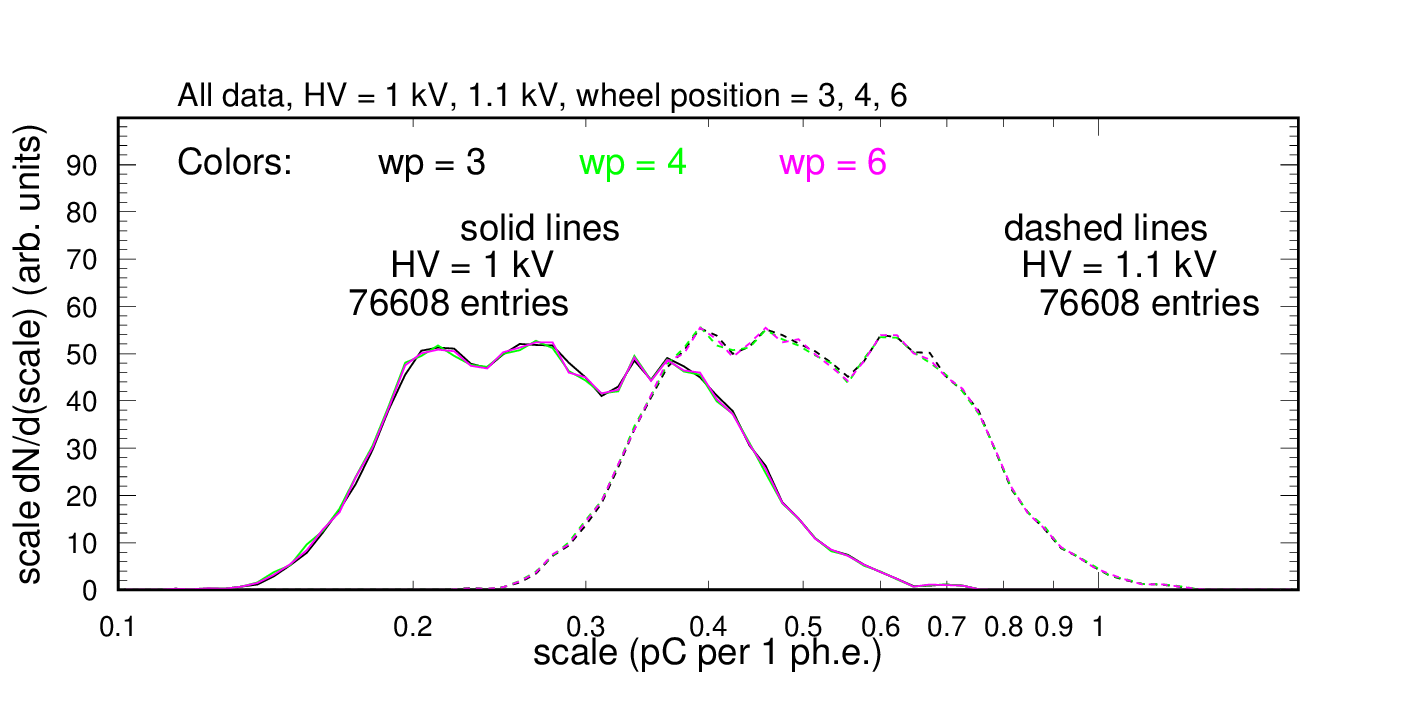
\includegraphics[width=0.98\linewidth,trim=0 15 50 35,clip]{figures/pglobal_sc.pdf}
	\caption{Distribution of $scale$ (average charge per ph.e) as determined by the fitting procedure for a set of 399 PMTs. All measured pixels contributed to the plots. Distributions measured at HV = 1000 V are shown by solid lines, the ones at HV = 1100 V by dashed lines. The three colors correspond to the three different illuminations (essentially on top of each other).
	}
	\label{fig:pglobal_sc}
\end{figure}

Fig. \ref{fig:pglobal_qe_all} shows the similar pattern for the $\mu$ parameter, with the difference that $\mu$ essentially does not depend on high voltage, but proportional to the light intensity. The plot shows that the distributions at different high voltages are on top of each other at a given light intensity, but shift in log scale when light intensity changes. In the plot the parameter $\mu$ is shown normalized to the number of photons coming to each pixel in the ``wheel position 3'' setting, to provide the value of quantum efficiency in it. 
\begin{figure}[hbt]
	\centering
	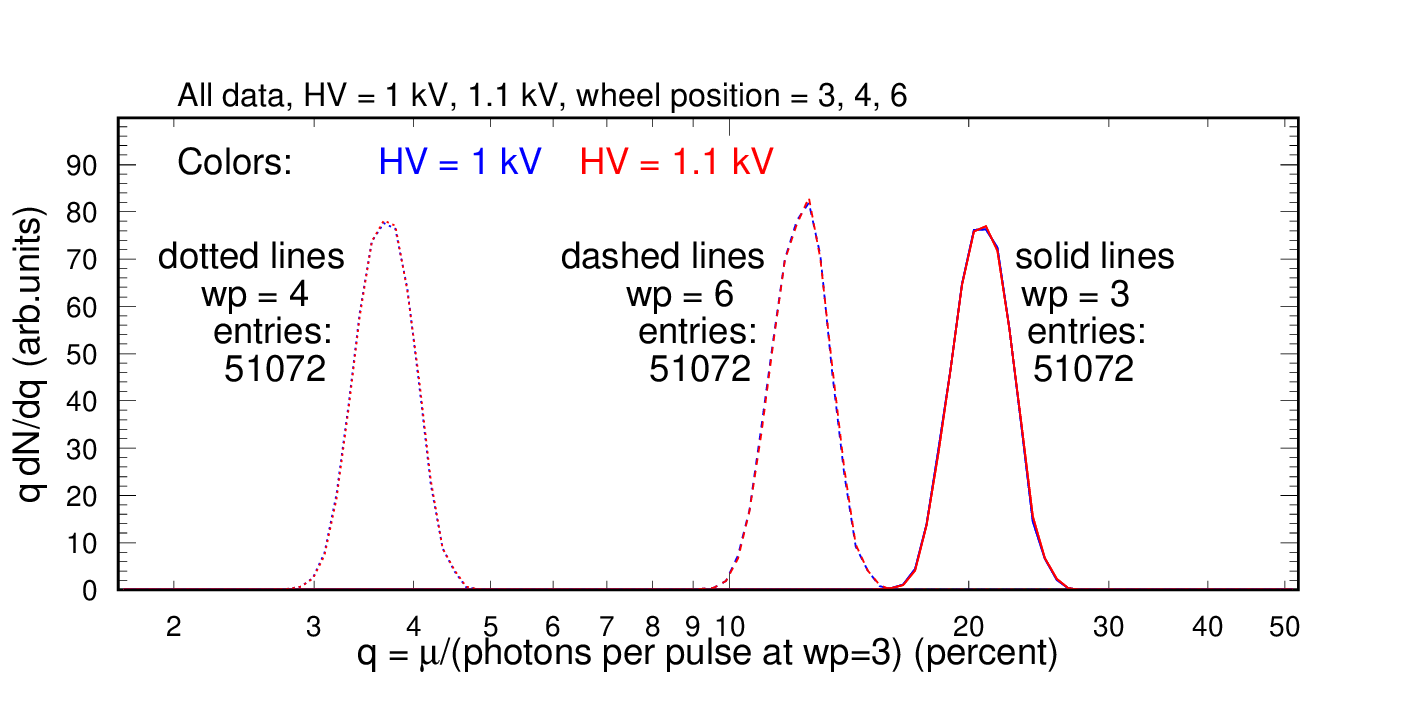
\includegraphics[width=0.98\linewidth,trim=0 15 50 35,clip]{figures/pglobal_qe_all.pdf}
	\caption{Distribution of $\mu$ divided by the measured number of photons per pulse at wheel position 3. All measured pixels contributed to the plots. Distributions measured at HV = 1000 V are shown by violet, the ones at HV = 1100 V by red color (essentially on top of each other). The three line styles (dotted, dashed, and solid) correspond to different illumination. For the data collected at wheel position 3, this ratio is the quantum efficiency of the individual pixels.}
	\label{fig:pglobal_qe_all}
\end{figure}
\begin{figure}[h!bt]
	\centering
	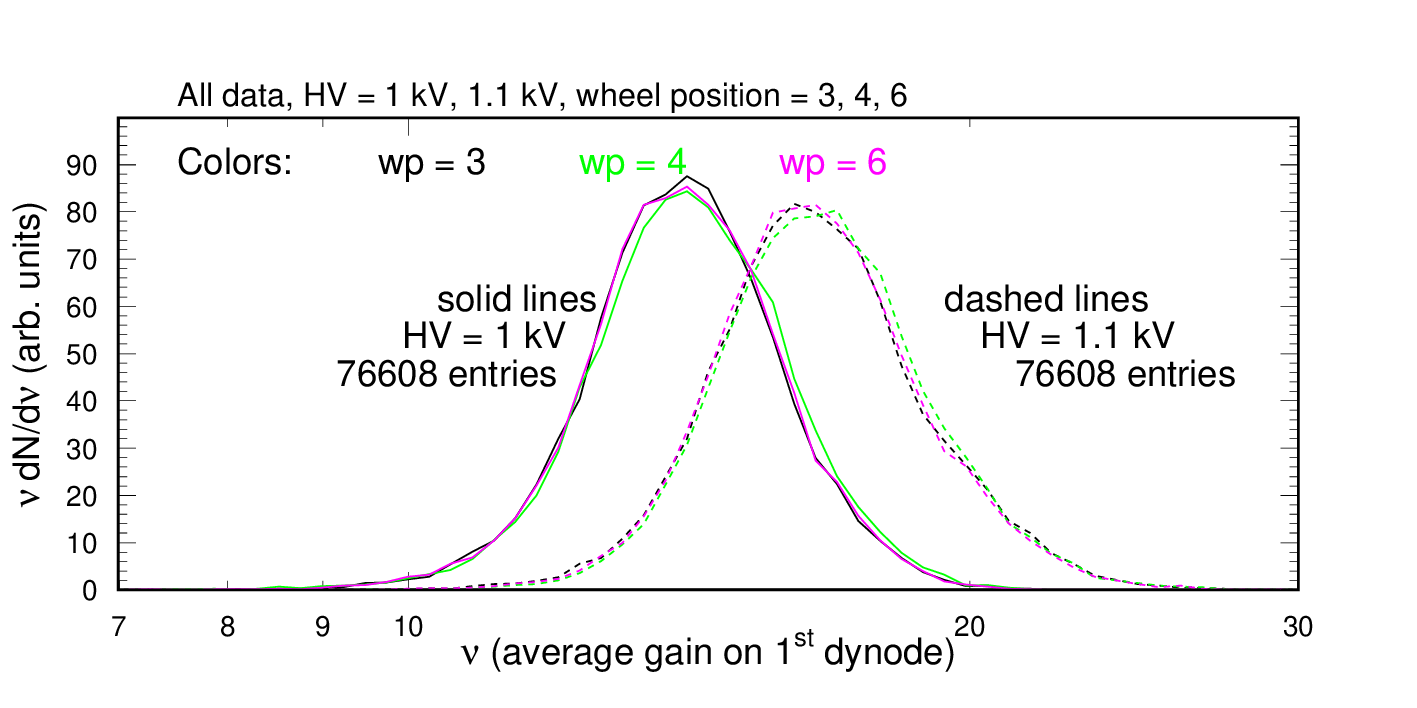
\includegraphics[width=0.98\linewidth, trim=0 15 50 35,clip]{figures/pglobal_nu.pdf}
	\caption{Distribution of $\nu$ (average gain on 1st dynode) as determined by the fitting procedure for a set of 399 PMTs.}
	\label{fig:pglobal_nu}
\end{figure}



\begin{figure}[h!bt]
	\centering
	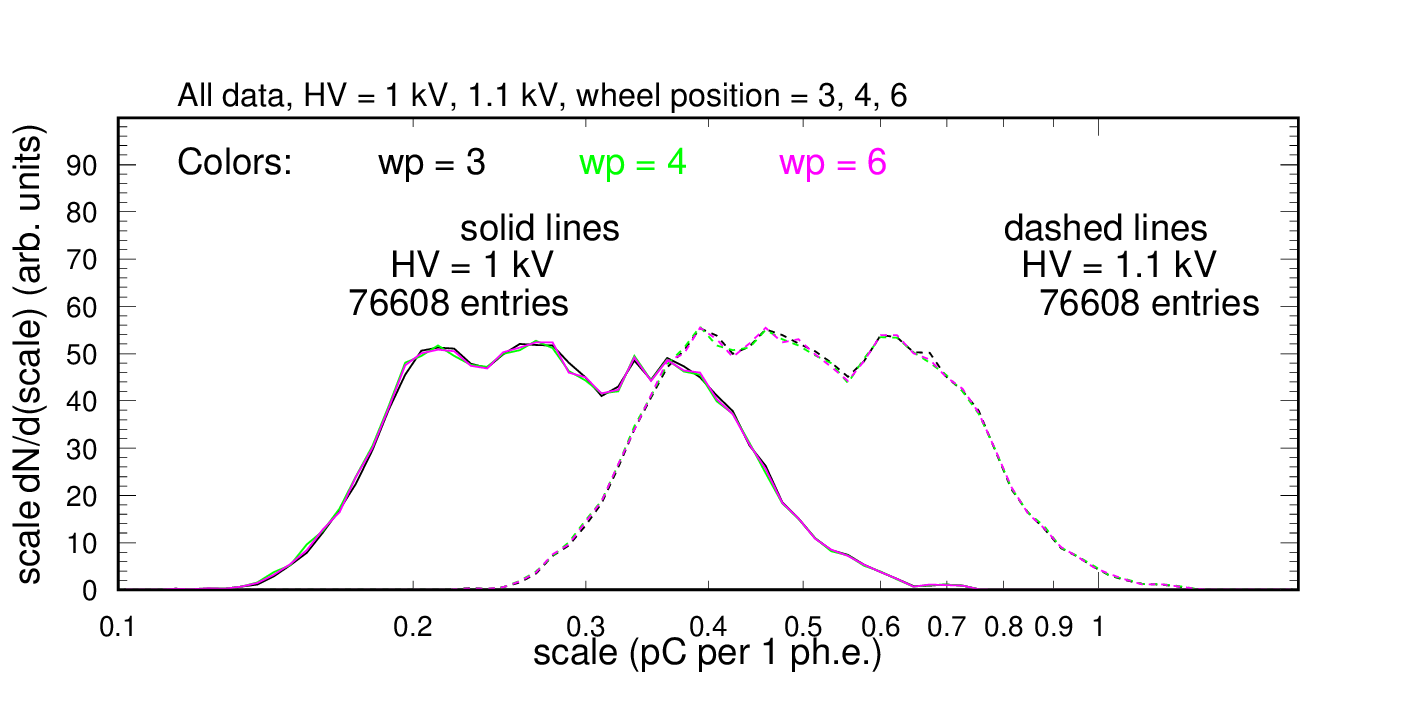
\includegraphics[width=0.98\linewidth, trim=0 15 50 35, clip]{figures/pglobal_sc.pdf}
	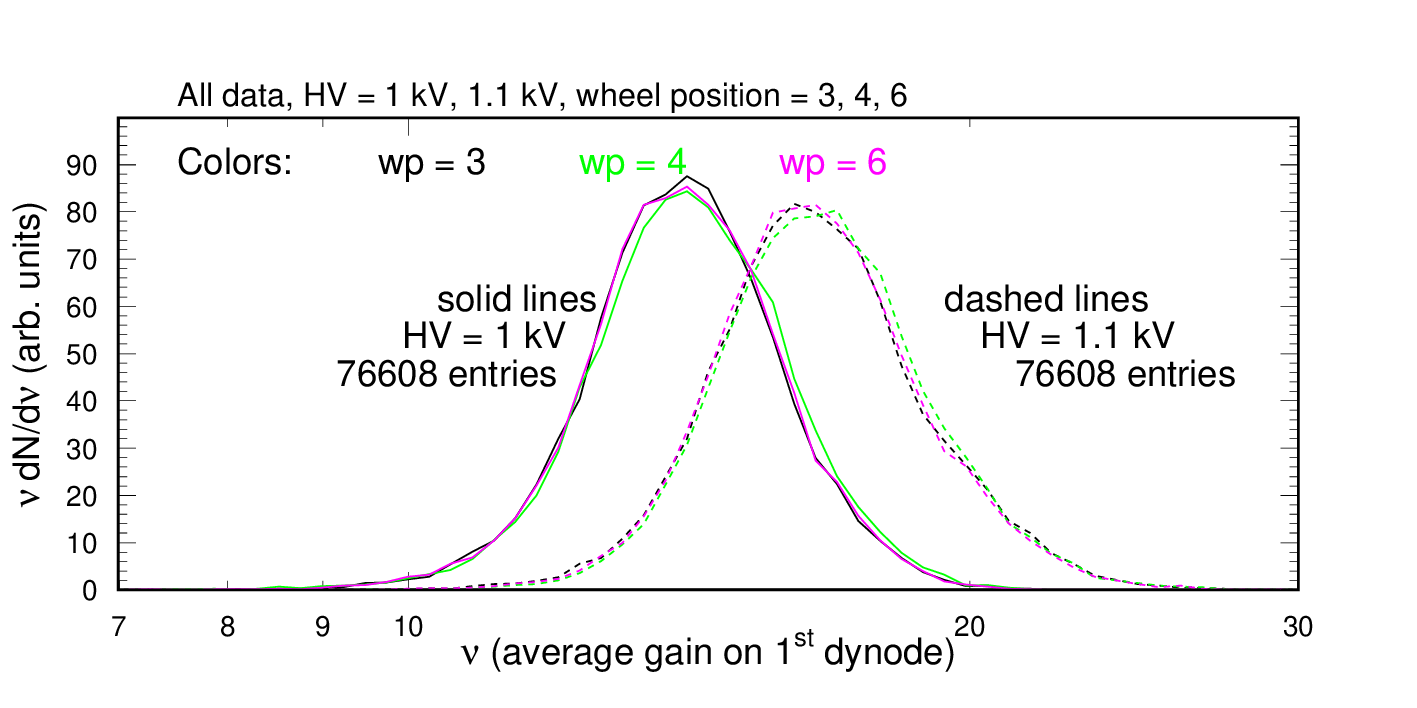
\includegraphics[width=0.98\linewidth, trim=0 15 50 35, clip]{figures/pglobal_nu.pdf}
	\caption{Distribution of scale (average charge per ph.e) and $\nu$ (average gain on 1st dynode) as determined by the fitting procedure for a set of 399 PMTs.}
	\label{fig:pglobal_sc_nu}
\end{figure}

\begin{figure}[h!bt]
	\centering
	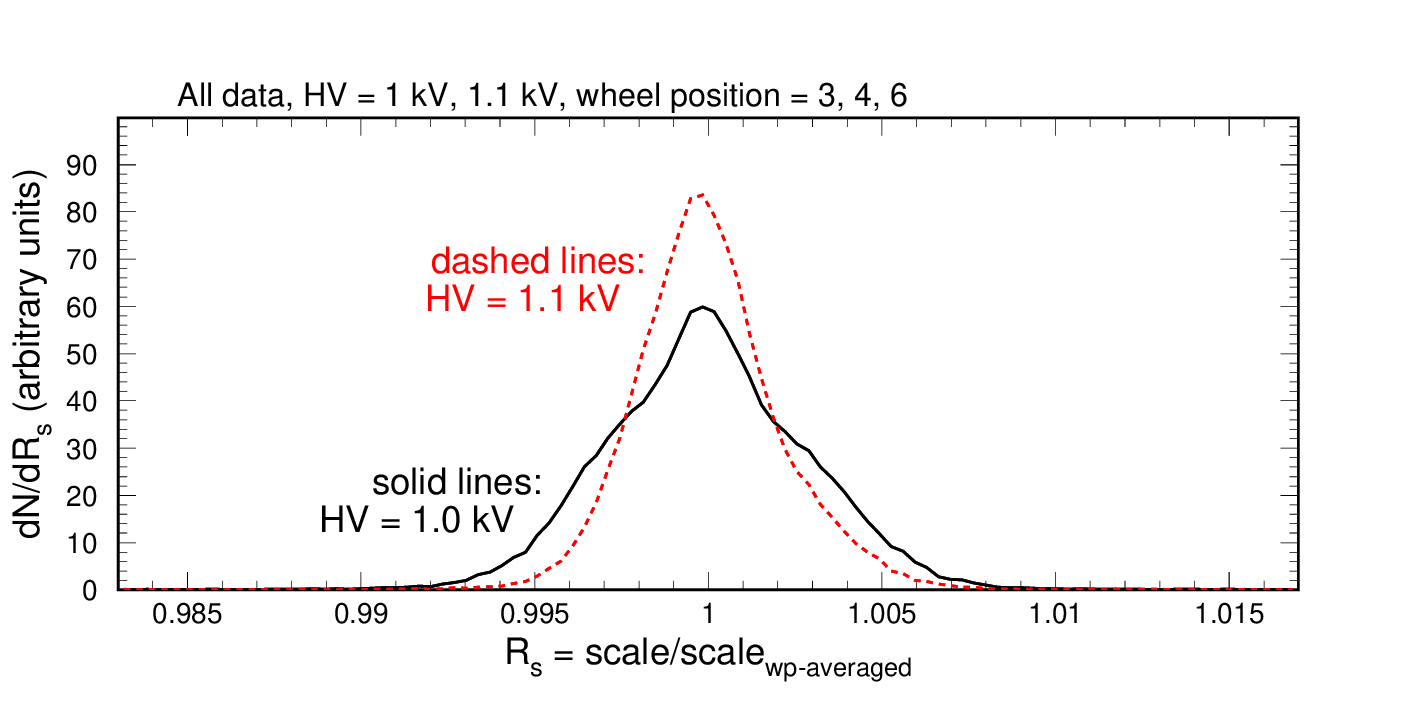
\includegraphics[width=0.98\linewidth, trim=0 15 50 35, clip]{figures/pglobal_Rs.pdf}
	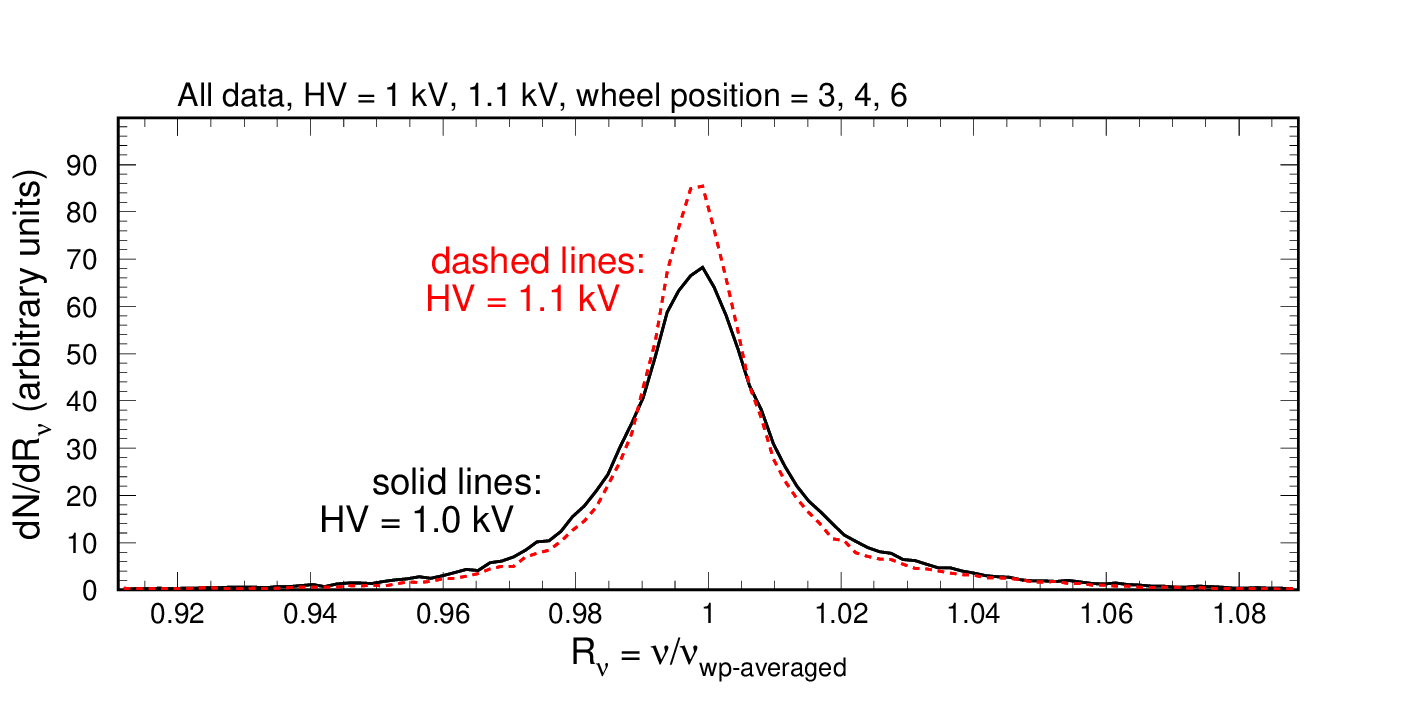
\includegraphics[width=0.98\linewidth, trim=0 15 50 35, clip]{figures/pglobal_Rn.pdf}
	\caption{Scale and $\nu$ averaged over three different illumination settings (wheel positions 3, 4, and 6).}
	\label{fig:pglobal_Rs_Rn}
\end{figure}

\begin{figure}[h!bt]
	\centering
	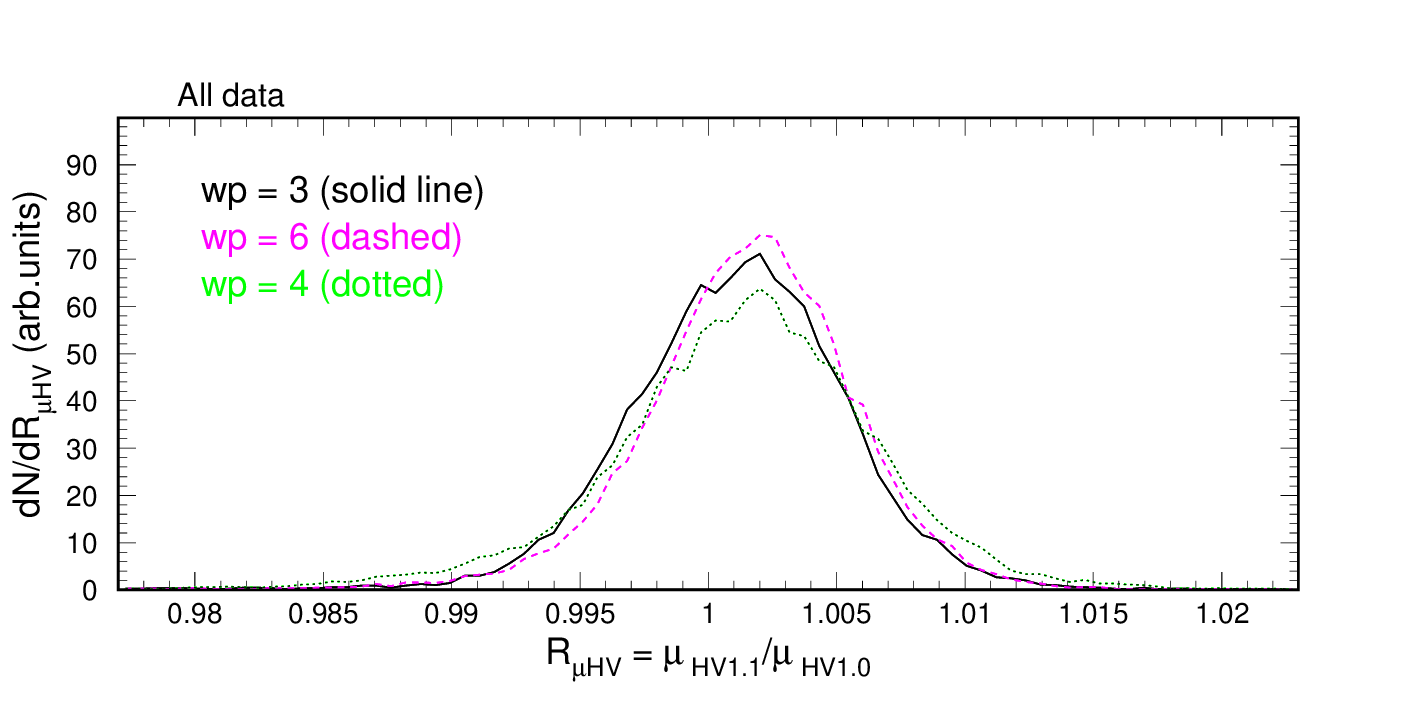
\includegraphics[width=0.98\linewidth, trim=0 15 50 35, clip]{figures/pglobal_mHV.pdf}
	\caption{The ratio of the $\mu$ parameters from the fit results at HV = 1100 V to the results at HV = 1000 V.}
	\label{fig:pglobal_mHV}
\end{figure}


\begin{figure}[h!bt]
	\centering
	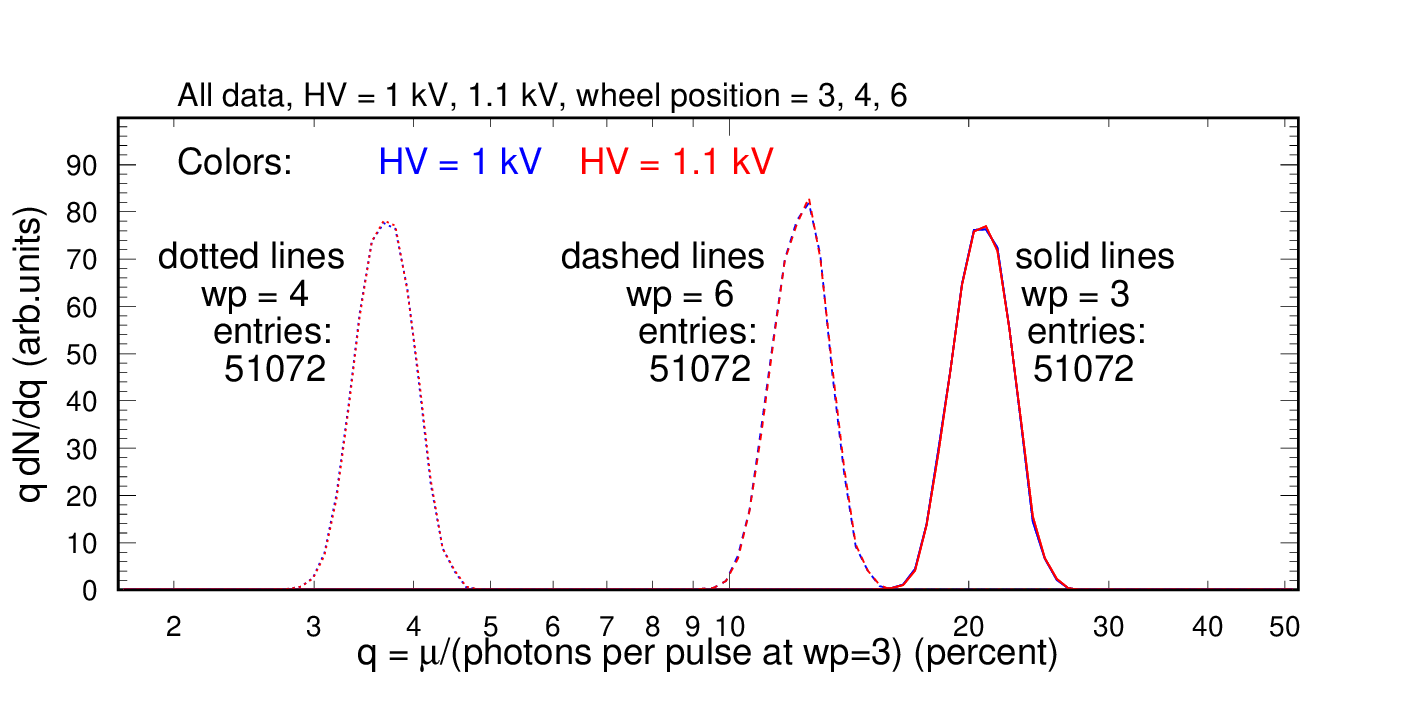
\includegraphics[width=0.98\linewidth, trim=0 15 50 35, clip]{figures/pglobal_qe_all.pdf}
	\caption{Distribution of $\mu$ divided by the measured number of photons per pulse at wheel position 3. For the data collected at wheel position 3, this ratio is the quantum efficiency of the individual pixels.}
	\label{fig:pglobal_qe_all}
\end{figure}

\begin{figure}[h!bt]
	\centering
	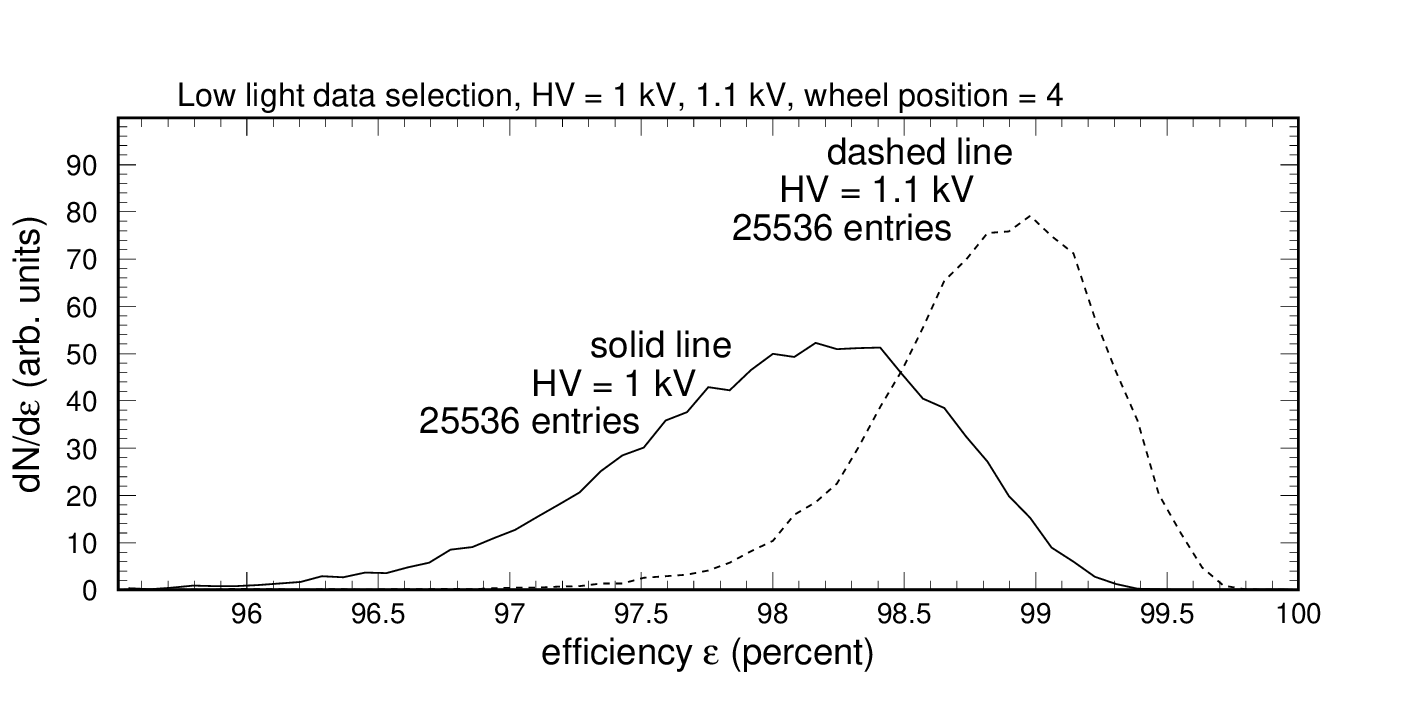
\includegraphics[width=0.98\linewidth, trim=0 15 50 35, clip]{figures/pglobal_eff.pdf}
	\caption{Distribution of the measured efficiency for all pixels at wheel position 4.}
	\label{fig:pglobal_eff}
\end{figure}

\begin{figure}[h!bt]
	\centering
	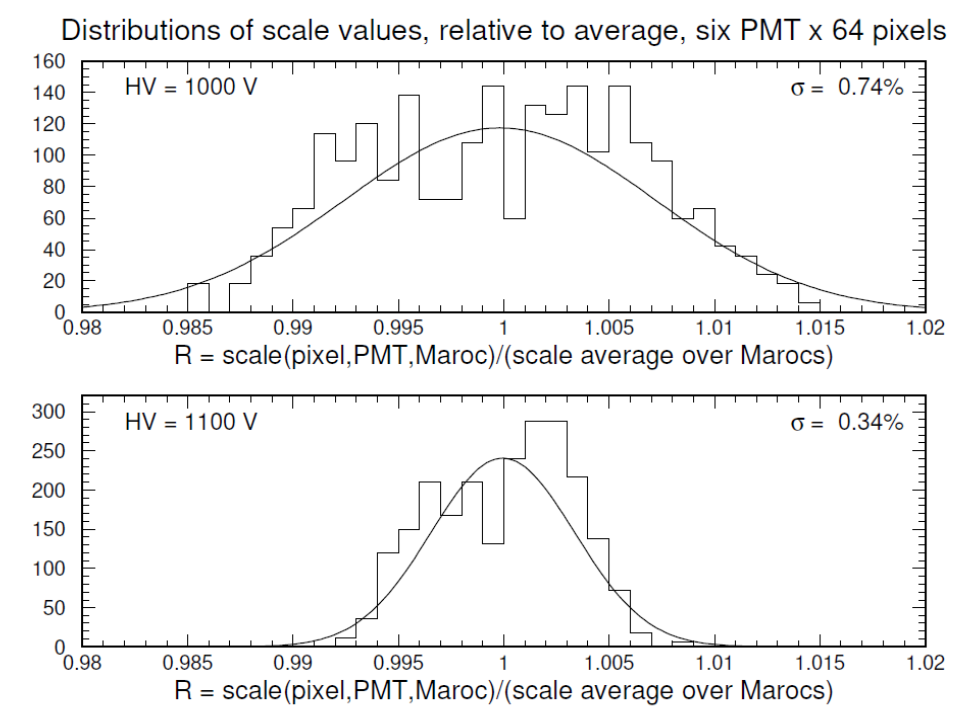
\includegraphics[width=0.98\linewidth, trim=0 10 15 10, clip]{figures/R_scale_maroc_avg.png}
	\caption{Evaluated precision of the scale parameter measurement for the two high voltage settings.}
	\label{fig:R_scale_maroc_avg}
\end{figure}


\begin{figure*}[hbt]
	\centering
	\begin{subfigure}[c]{0.4\linewidth}
		\centering
		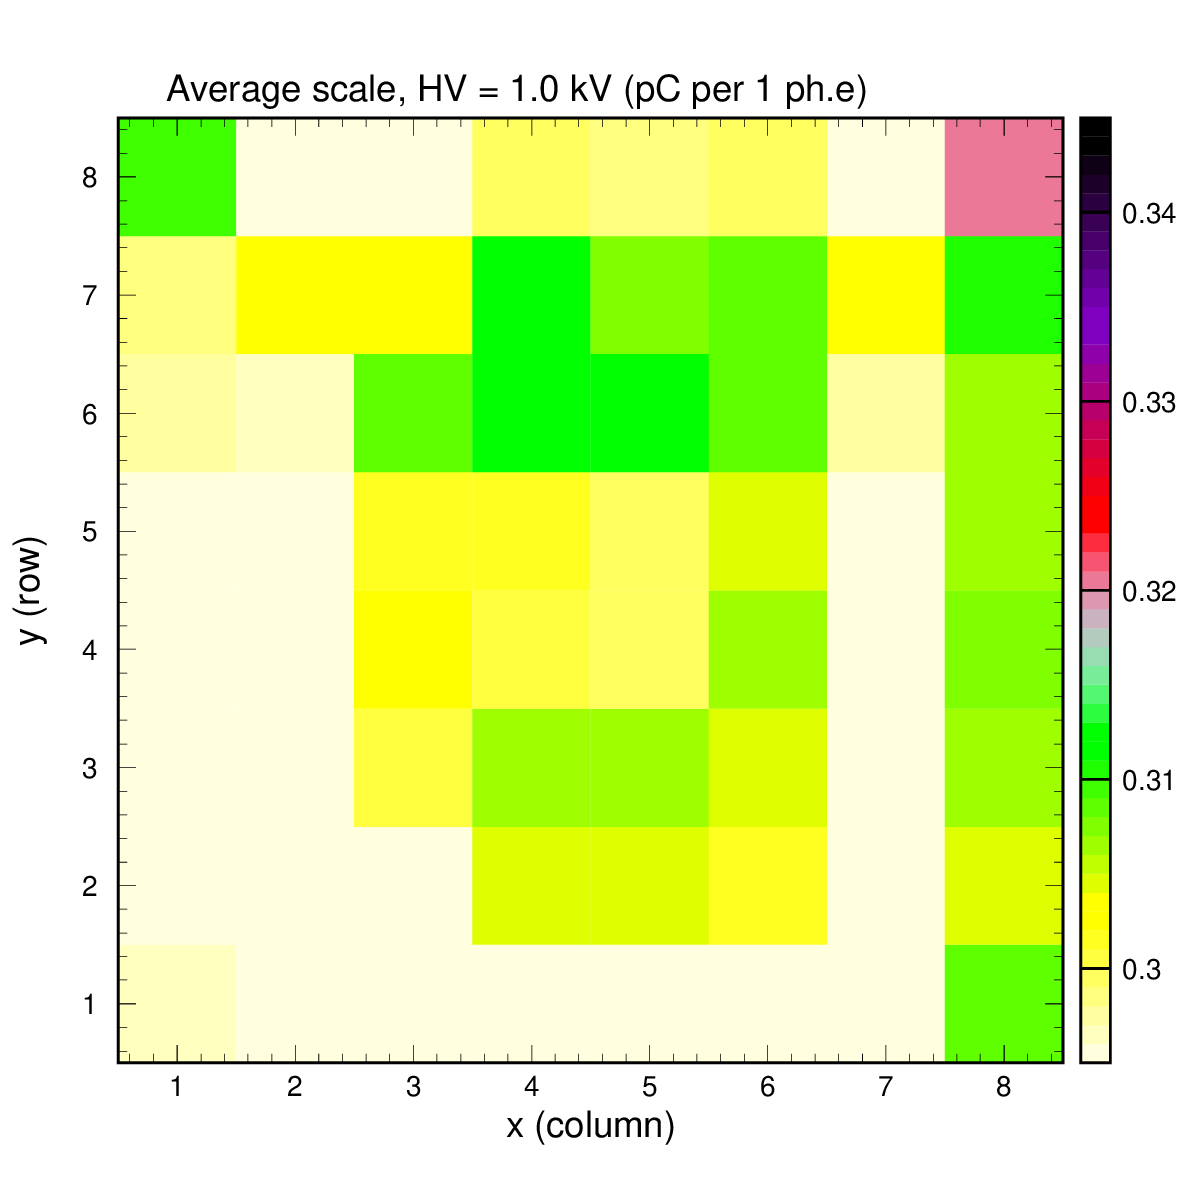
\includegraphics[width=\linewidth, trim={0mm 0mm 0mm 19mm},clip]{figures/pglobal_sc2d.pdf}
		\caption{Average scale, HV = 1.0 kV (pC per 1 ph.e)}
		\vspace{0mm}
	\end{subfigure}%%
	\begin{subfigure}[c]{0.4\linewidth}
		\centering
		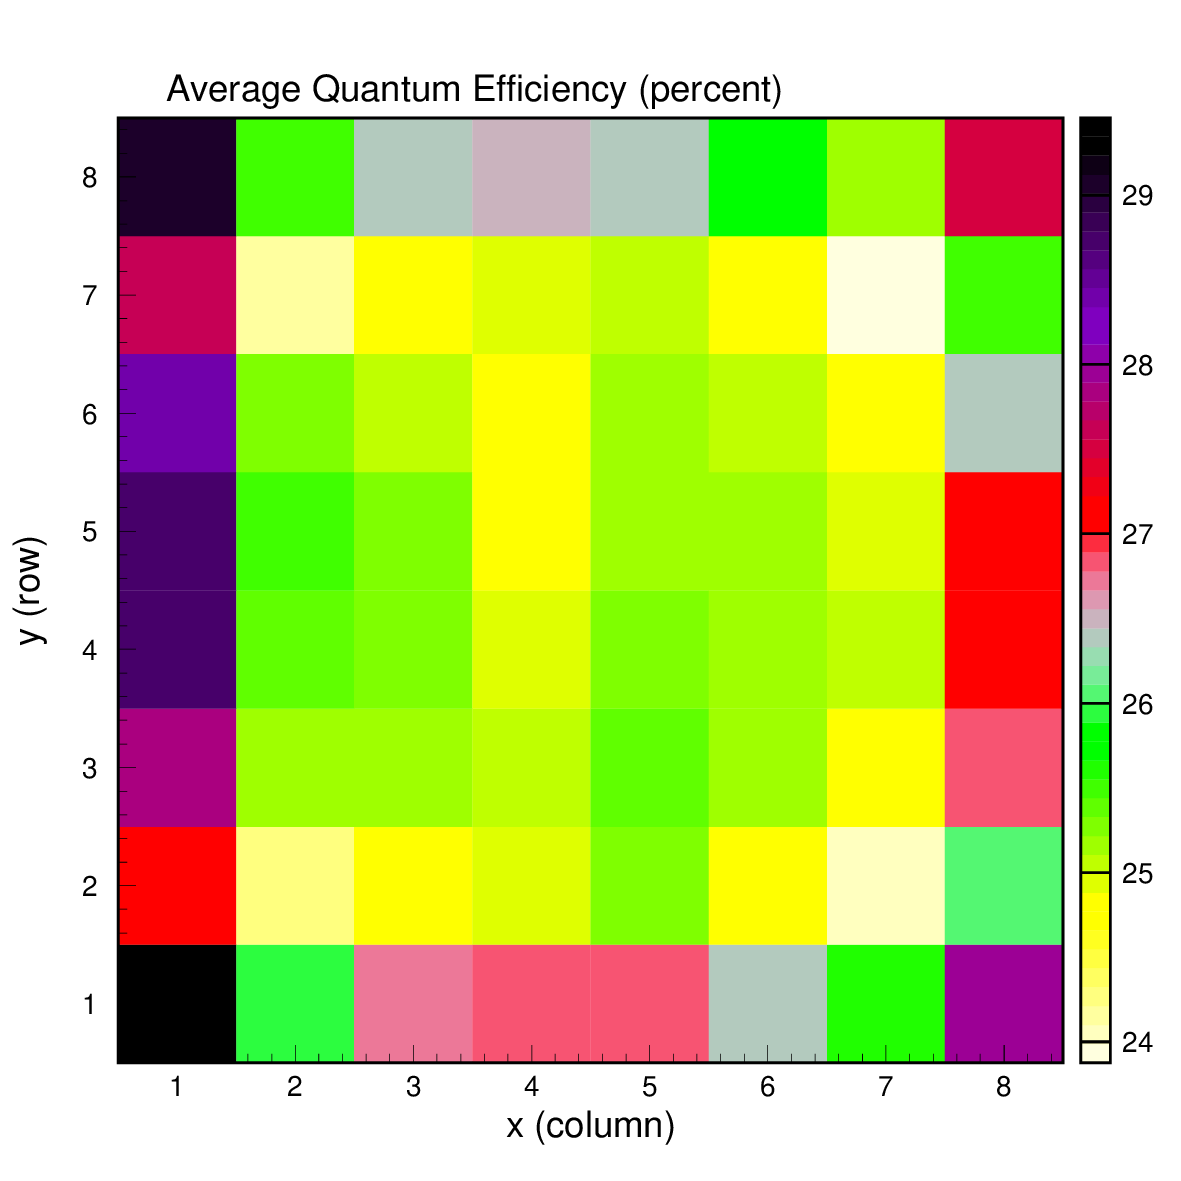
\includegraphics[width=\linewidth, trim={0mm 0mm 0mm 19mm},clip]{figures/pglobal_qe.pdf}
		\caption{Average Quantum Efficiency (percent)}
		\vspace{0mm}
	\end{subfigure}%%
	\vspace{3mm}
	\begin{subfigure}[c]{0.4\linewidth}
		\centering
		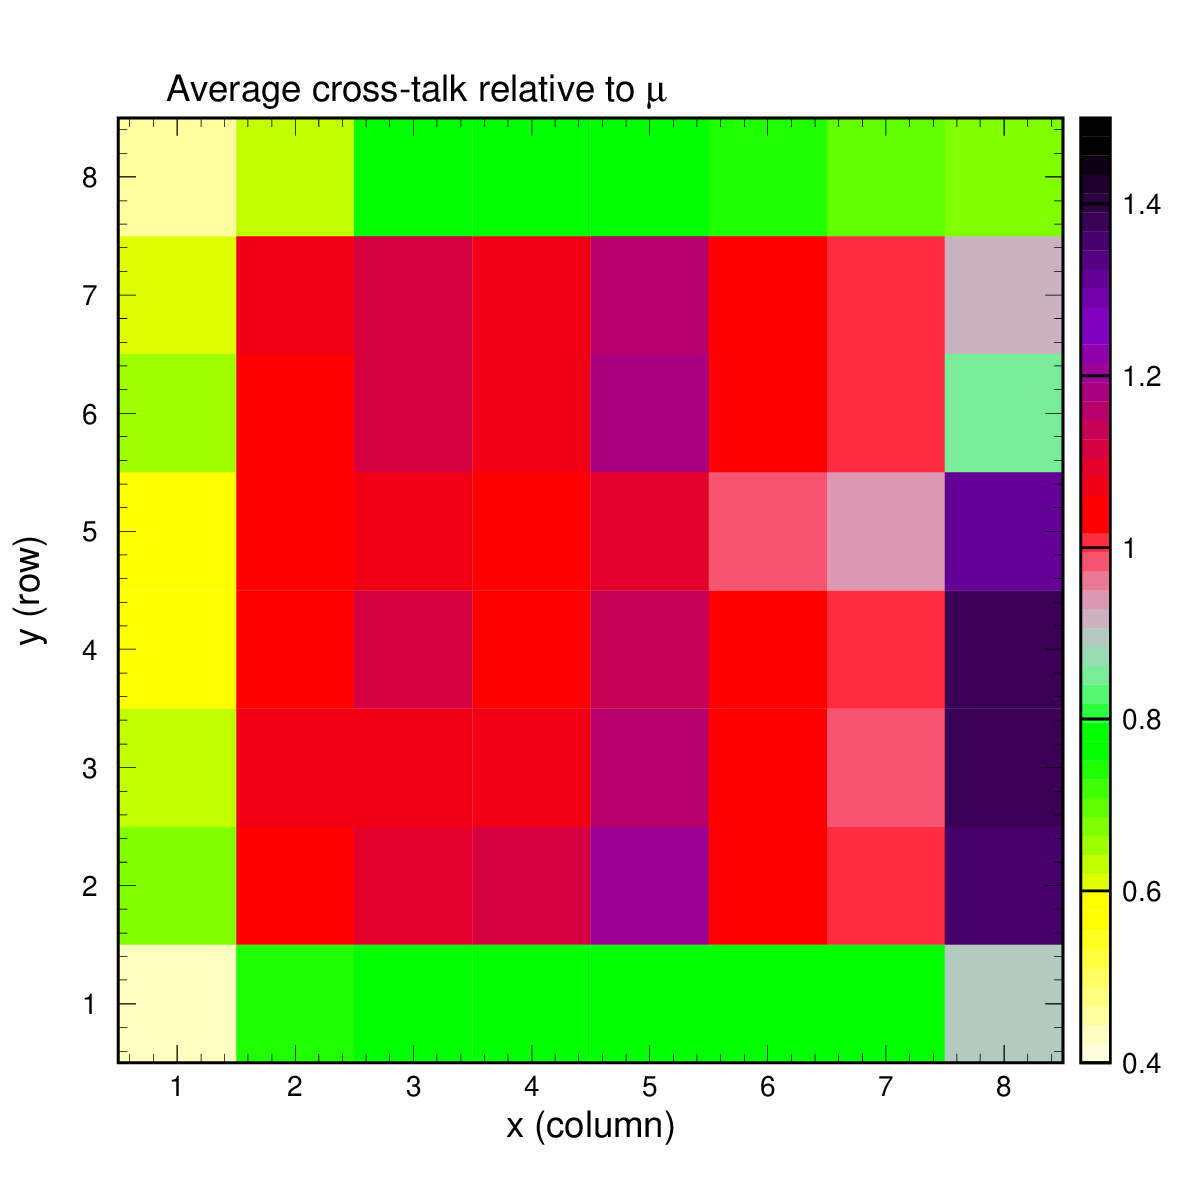
\includegraphics[width=\linewidth, trim={0mm 0mm 0mm 19mm},clip]{figures/pglobal_beta.pdf}
		\caption{Average cross-talk relative to $\mu$}
		\vspace{0mm}
	\end{subfigure}%%
	\begin{subfigure}[c]{0.4\linewidth}
		\centering
		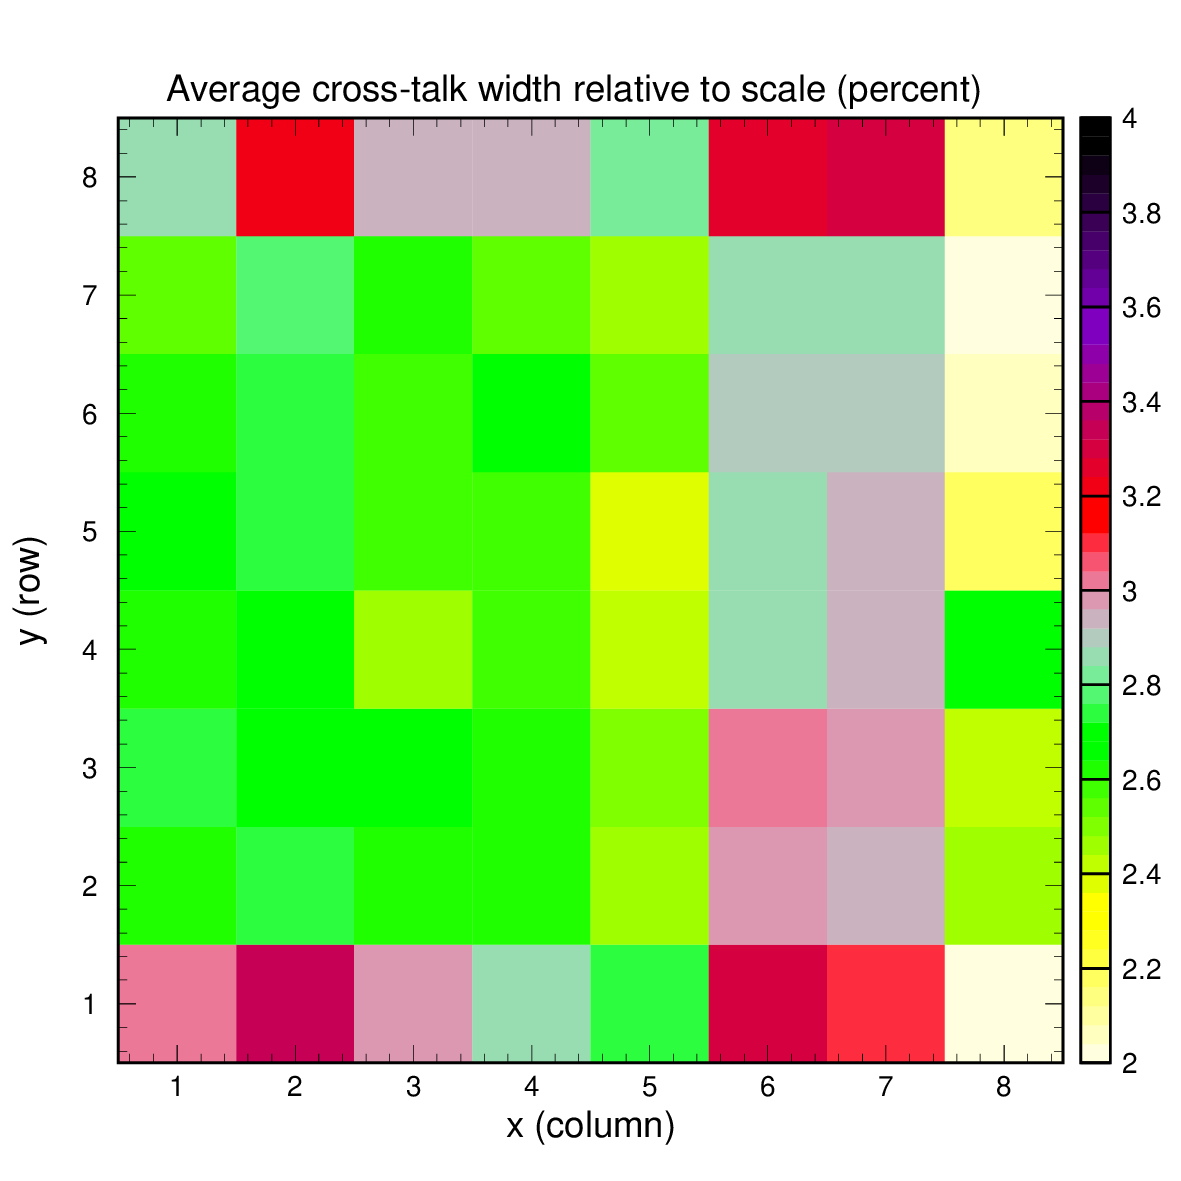
\includegraphics[width=\linewidth, trim={0mm 0mm 0mm 19mm},clip]{figures/pglobal_zeta.pdf}
		\caption{Average cross-talk width relative to scale (percent)}
		\vspace{0mm}
	\end{subfigure}%%
	\vspace{3mm}
	\begin{subfigure}[c]{0.4\linewidth}
		\centering
		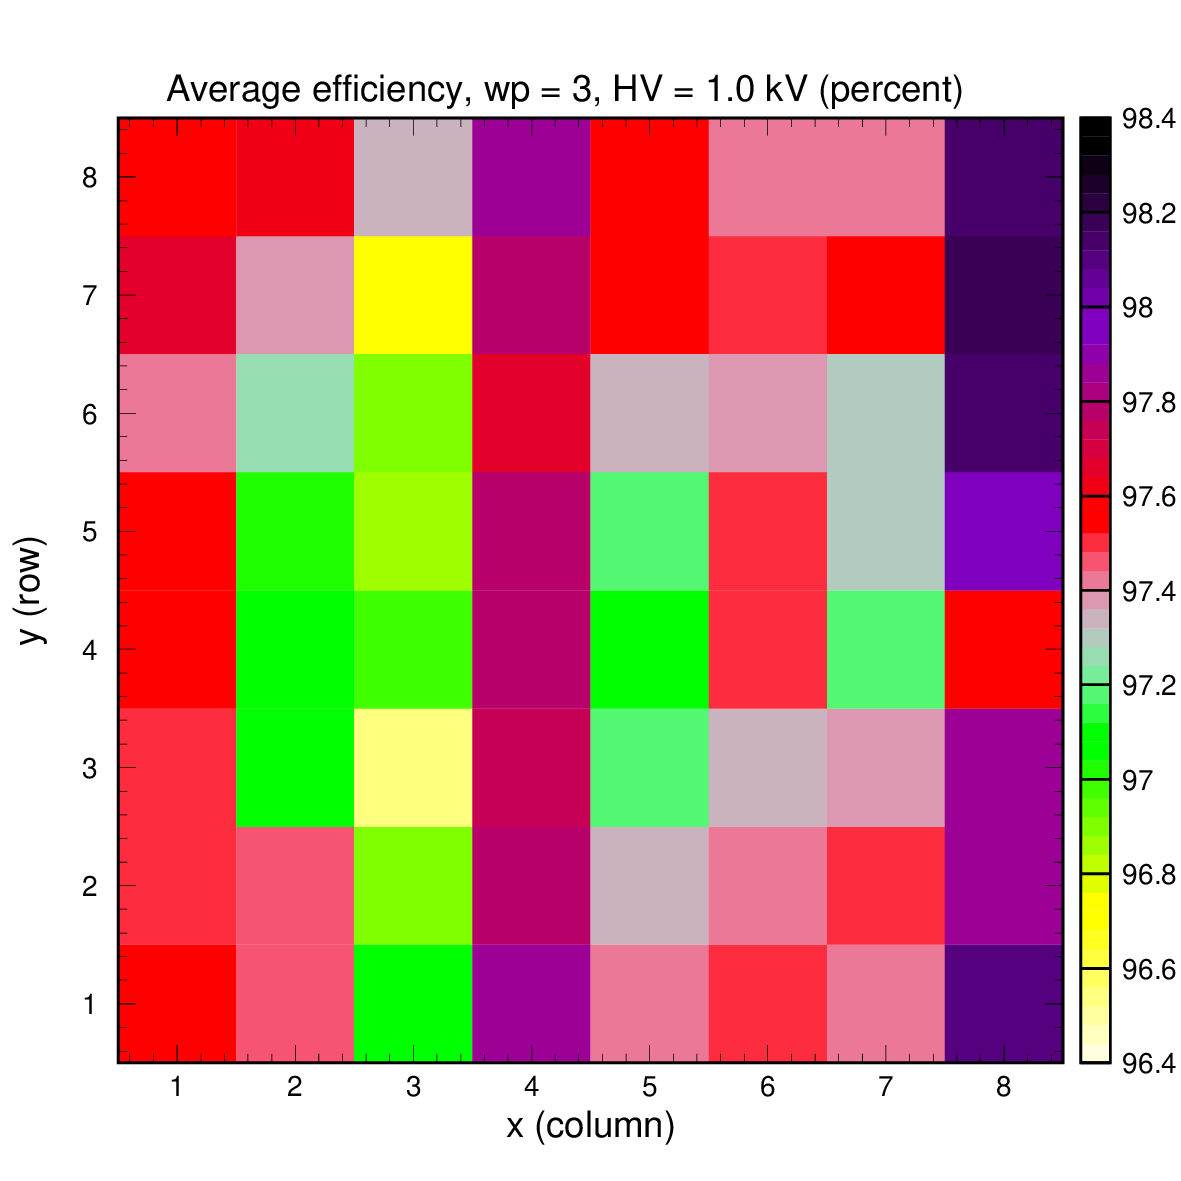
\includegraphics[width=\linewidth, trim={0mm 0mm 0mm 19mm},clip]{figures/pglobal_eff2d.pdf}
		\caption{Average efficiency, wp = 3, HV = 1.0 kV (percent)}
		\vspace{0mm}
	\end{subfigure}%%
	\caption{Two dimensional plots showing the average (a) scale, (b) quantum efficiency, (c) cross-talk relative to $\mu$, (d) cross-talk relative to scale, and (e) efficiency as a function of pixel location.}
	\label{fig:2d_avg_fit_results}
\end{figure*}



Large number of MAPMTs from Hamamatsu (XX of H8500 type, and XXX of H12700 type) were studied using the dedicated test stand at JLab. Their performance as single photon detectors was evaluated and characterized in conditions close to their future operations in the CLAS12 RICH detector.


Parameters of the single photoelectron response function of every pixel were extracted using the SPE spectra approximations in our mathematical model, modified to take into account the effects of the signal cross-talk between the neighboring pixels. The stability and consistency of the parameter values measured in different conditions of illumination and at different applied high voltages allows to characterize the intrinsic features of every pixel, independent on the measurement conditions. Absolute quantum efficiency and electronic gain of every channel, as well as the set of parameters describing variable shapes of the SPE functions were measured.


The parameter database accumulated as the result of this work was used for the selection of the PSPMTs for installation in the RICH detector, and for the optimization of the future run parameters, such as the tube placement selection, setting the values of operating high voltage, electronics gains and thresholds in the detector.


The data also provide the opportunity to evaluate the spread of such parameters in the mass production of the PSPMT devices as the channel gains, quantum efficiencies, SPE spectral shapes, parameters of the cross-talk, - across the face of each tube, and across the whole set. The results show that the quality of PSPMT mass production at Hamamatsu is high and satisfies our needs in the good quality single photoelectron detection.



%We saw that although there is little difference in crosstalk signals, the H12700 PMTs suffer less from dark current, have narrower SPE spectra, and have higher $\mu$ and relative efficiency values.
%An example plot of the $\mu$'s and relative efficiencies of H8500 and H12700 PMTs with similar low and high gains is shown in Figure \ref{efficiency}.

%We see that the relative efficiency is closely related to the $\mu$ which is on average, over all pixels at all voltages for all the PMTs we tested, $29\pm5$ percent higher in H12700 than H8500 MAPMTs. One concern with these $\mu$ measurements however is that the laser system used to measure these PMTs was only incident on a portion of each pixel, consequently missing their sum total effect and pinpointing possible spatial dependencies which should be further studied and perhaps remeasured with a fully illuminated MAPMT instead of collimated pinpoint laser light. In terms of crosstalk for the two varieties of MAPMT the H12700s appear to be better than the H8500s. The H12700s have a decrease in crosstalk by nearly a factor of two. Additional studies of dark current in the H12700s would be useful, as the dark current is usually dominated by individual pixels or bad regions of the PMT instead of spread around evenly like in the H8500s, but overall the two varieties are not very different in terms of dark current.